If instead we sample a grid of points on the Poincar\'e section $\Sout$, we can compute LZ as in \cref{subfig:LZpoincaresectionb3}. We only compute LZ for a strip of the Poincar\'e section, specifically, for $\theta\in[-\pi/4,\pi/4]$, since the rest of the picture can be reconstructed via translation. This corresponds to the 4-fold rotational symmetry of a square lattice, that is, if we rotate $\mathbb R^2$ at the origin by an angle of $n*\pi/2$ for $n=0,\dots, 3$, the lattice of circles stays the same, and the resulting dynamics are the same as well.

In \cref{subfig:LZpoincaresectionb3} we compute LZ for $R=1/3$ and $b=3$. We see a large stable ``eye'' at $(\theta, \varphi)=(0,0)$. This is not unexpected, since we've seen evidence for a large stable region in \cref{subfig:LZsweepY}. Besides the eye, we see some lines that have intermediate complexity, and on those either lie unstable periodic orbits or special occurances like \cref{fig:sensitive_trajectory}. We include some close ups of the eye: the top left corner of the eye where we notice some obvious fractal behavior, and another spot along the boundary of the eye. We must note again that the emerging features in the images are sensitive to varying the depth of simulation. When attempting to plot the close ups, for example, the second one, we noticed that more yellow strips would appear and their width would increase the longer we simulated. The deeper we simulate, the more the boundary moves, which is not unreasonable since we capture more information.

\begin{figure}[!th]
\centering
\hfill
\begin{subfigure}[h]{0.49\textwidth}
\centering
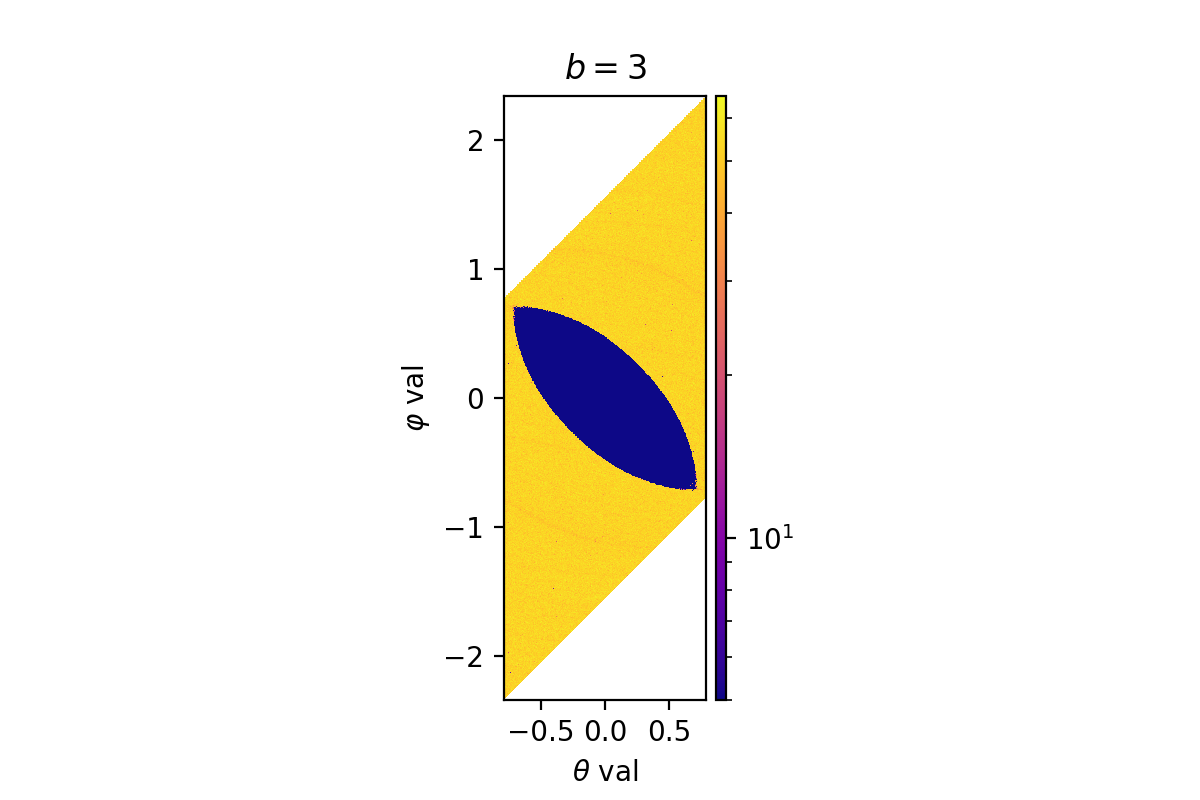
\includegraphics[width=\textwidth, trim={5cm 0cm 4cm 0cm}, clip]{LZ_th_ph_b_3_sweep.png}
\caption{}
\label{subfig:LZpoincaresectionb3}
\end{subfigure}
%
\begin{subfigure}[h]{0.49\textwidth}
\centering
%\includegraphics[width=\textwidth, trim={0cm 0 0cm 0}, clip]{fig18.png}
%
%\includegraphics[width=\textwidth, trim={0cm 0 0cm 0}, clip]{fig16.png}
%
%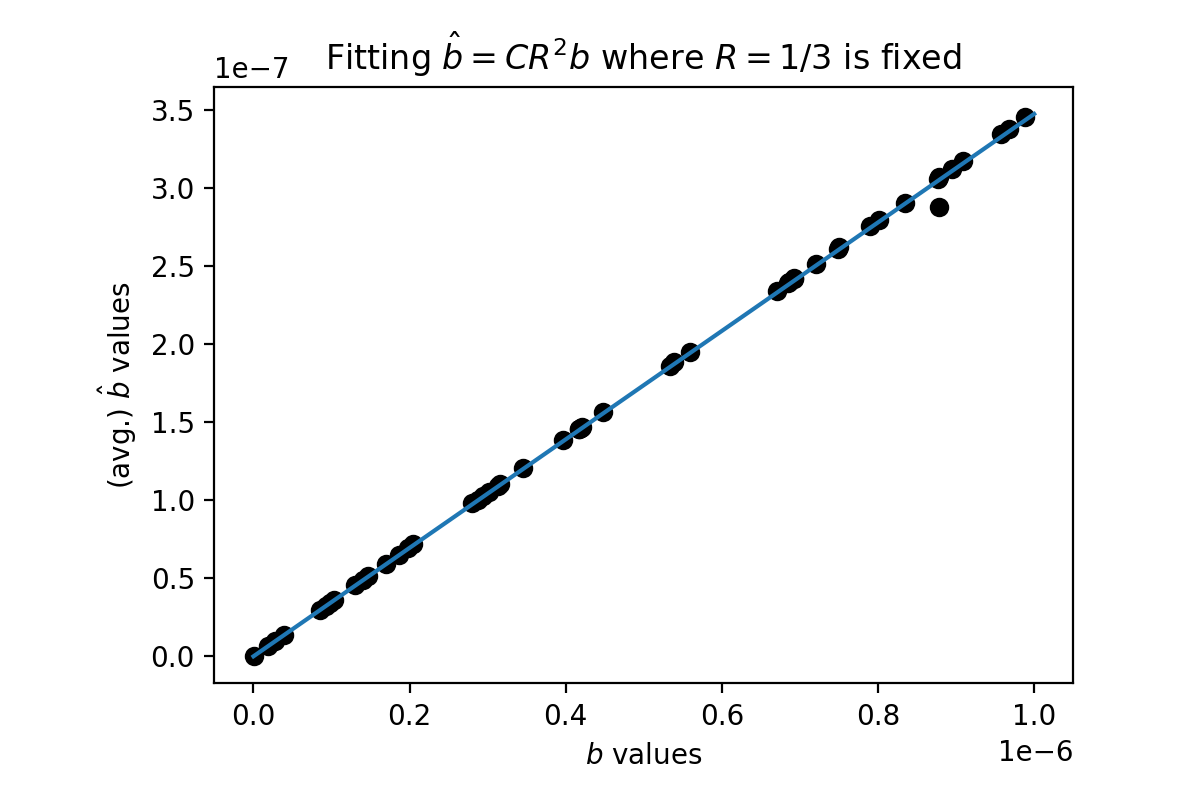
\includegraphics[width=\textwidth, trim={0cm 0 0cm 0}, clip]{kam_approx_line.png}
\caption{placeholder}
\end{subfigure}
\caption{}
\end{figure}


In \cref{subfig:LZpoincaresectionb1242} we plot the same data except $b\approx3(\sqrt2-1)$, so we plot the Poincar\'e section corresponding to \cref{subfig:periodicorbit3}. We notice there are several very stable regions, however by comparing with \cref{subfig:periodicorbit3} they should correspond to the same family of (quasi)-periodic orbits. The shape of the very stable regions is quite different, they are twisted with fractal ``digits''. Besides the large regions there are intermediate complexity regions scattered about, due to their globular shapes we suspect they are also relatively stable.

\begin{figure}[!th]
\centering
\hfill
\begin{subfigure}[h]{0.49\textwidth}
\centering
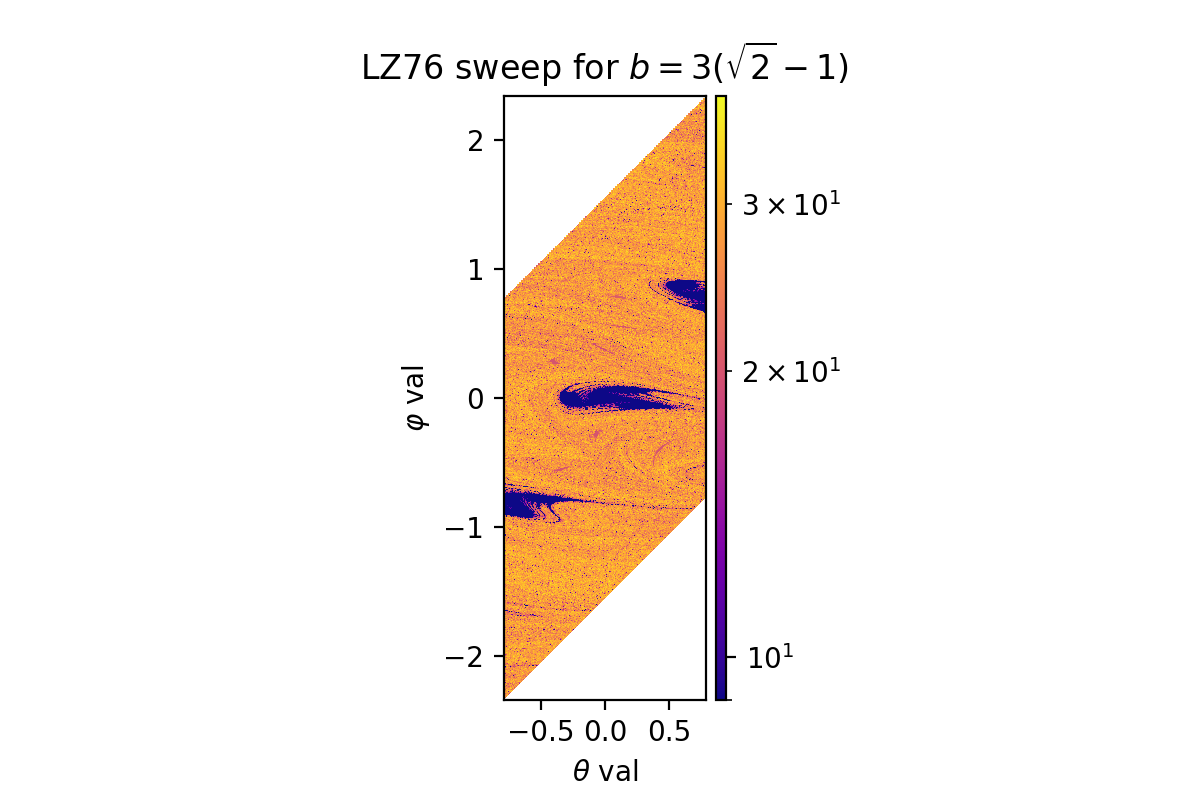
\includegraphics[width=\textwidth, trim={4cm 0cm 4cm 0cm}, clip]{LZ_th_ph_b_3sqrt2-1_sweep.png}
\caption{}
\label{subfig:LZpoincaresectionb1242}
\end{subfigure}
%
\hfill
\begin{subfigure}[h]{0.49\textwidth}
\centering
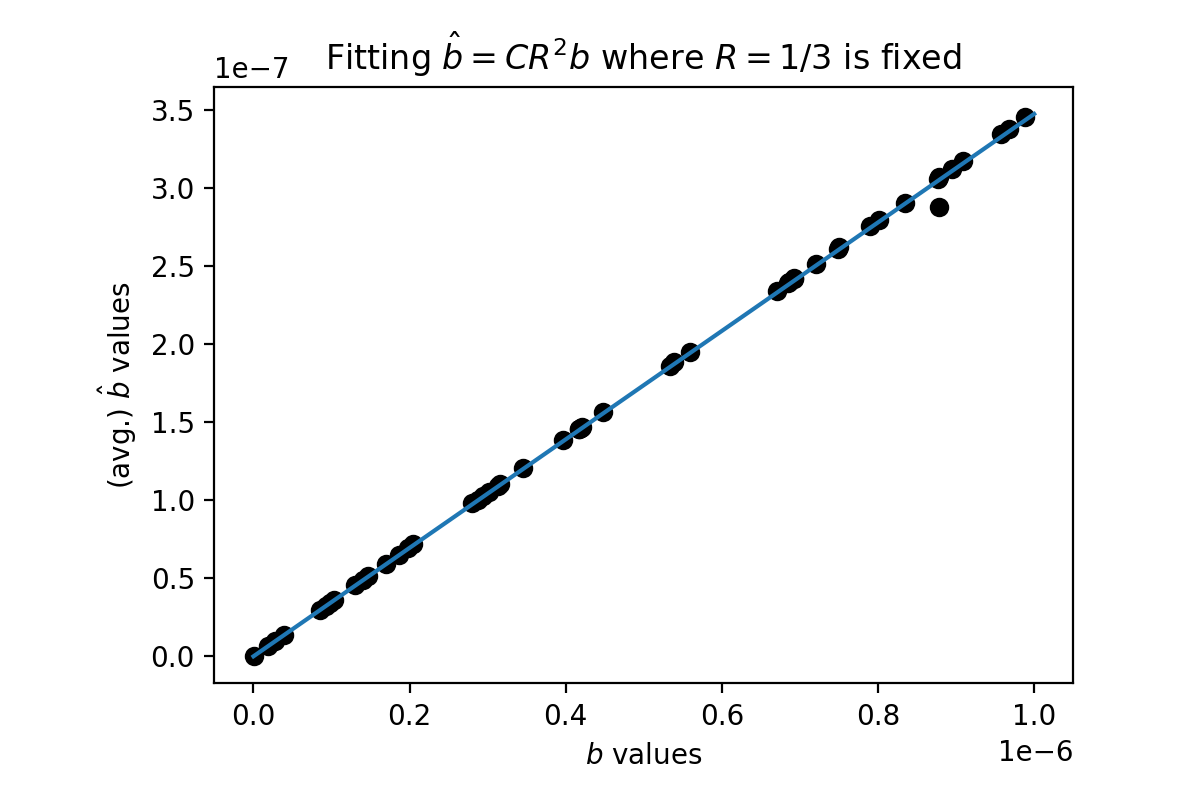
\includegraphics[width=\textwidth, trim={0cm 0 0cm 0}, clip]{kam_approx_line.png}
%
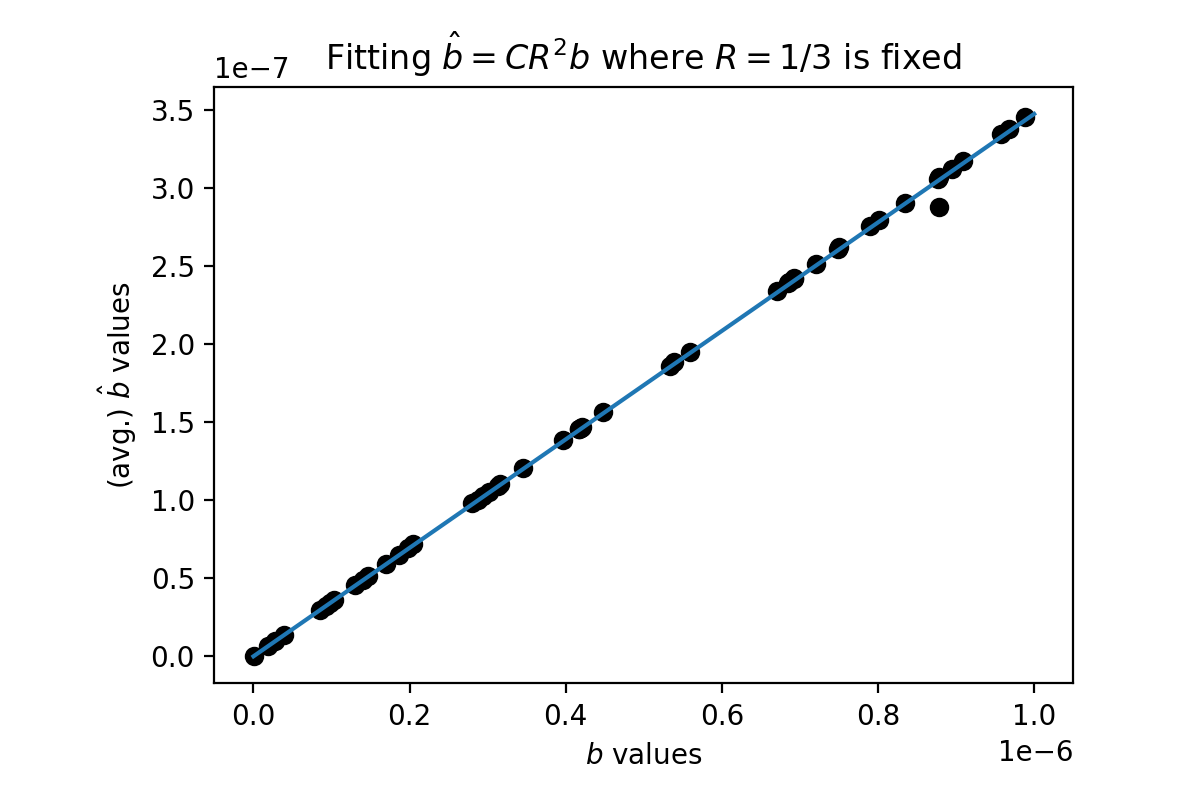
\includegraphics[width=\textwidth, trim={0cm 0 0cm 0}, clip]{kam_approx_line.png}
%
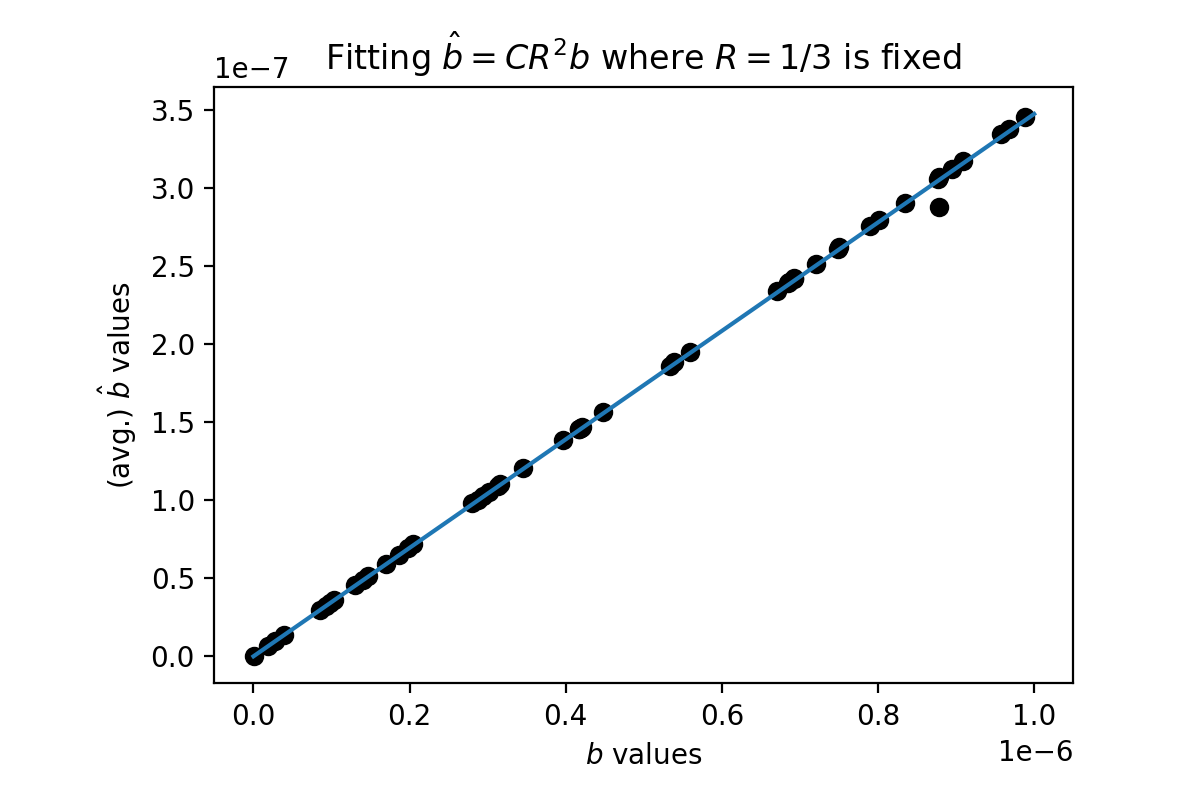
\includegraphics[width=\textwidth, trim={0cm 0 0cm 0}, clip]{kam_approx_line.png}
\caption{placeholder}
\end{subfigure}
\hfill
\caption{}
\end{figure}

In \cref{subfig:LZpoincaresectionb232}, we pick a value of $b=2.32$ and find a range of stable regions. Generally, the shapes are elongated, exaggerated compared to the other figures and it is not clear why this is the case. It can be noticed that there are 3 different colors for the stable regions, indicating there could be 3 different stable orbits here.

\begin{figure}[!th]
\centering
\hfill
\begin{subfigure}[h]{0.49\textwidth}
\centering
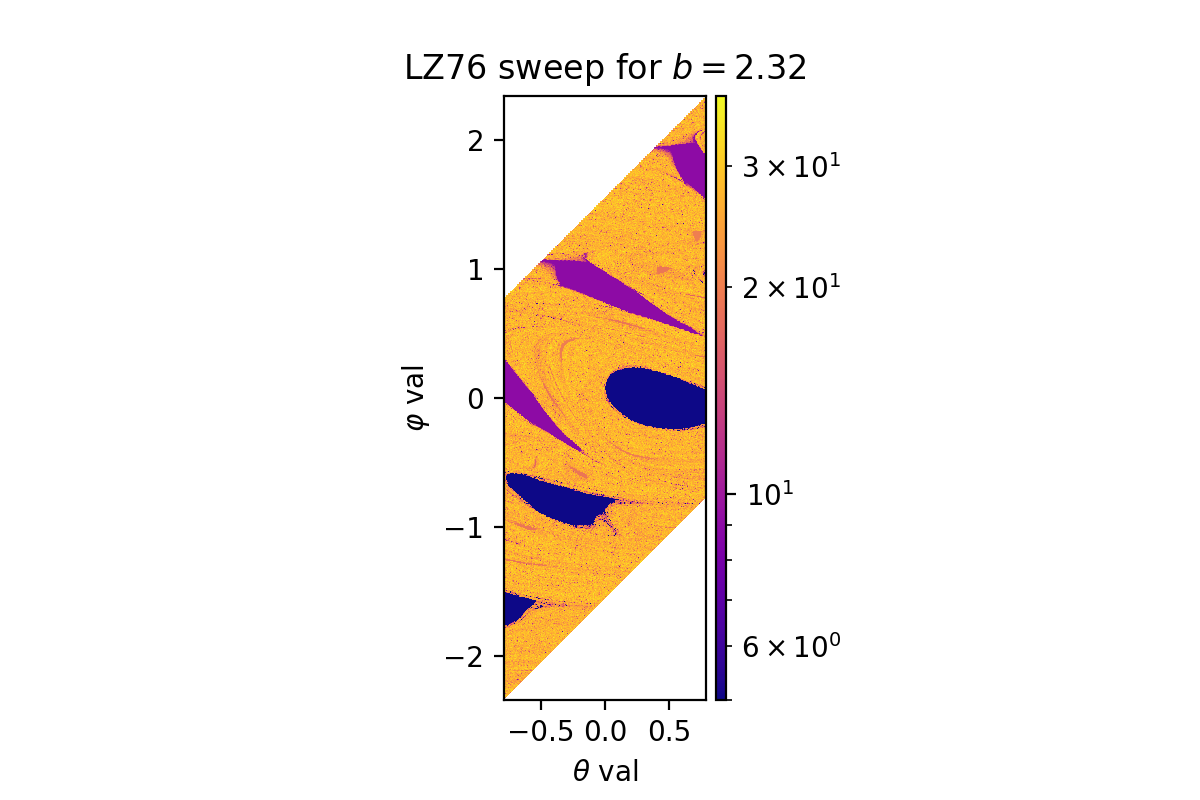
\includegraphics[width=\textwidth, trim={5cm 0cm 4cm 0cm}, clip]{LZ_th_ph_b_2_32_sweep.png}
\caption{}
\label{subfig:LZpoincaresectionb232}
\end{subfigure}
%
\hfill
\begin{subfigure}[h]{0.49\textwidth}
\centering
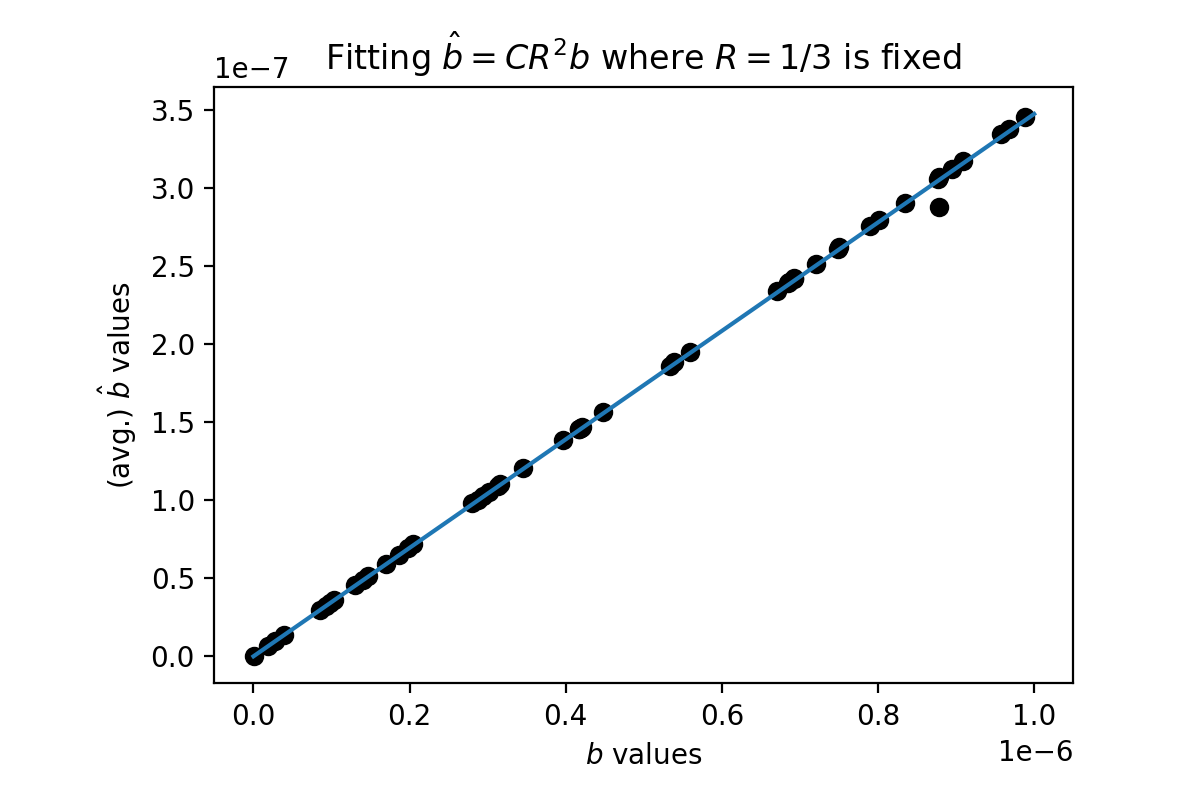
\includegraphics[width=\textwidth, trim={0cm 0 0cm 0}, clip]{kam_approx_line.png}
%
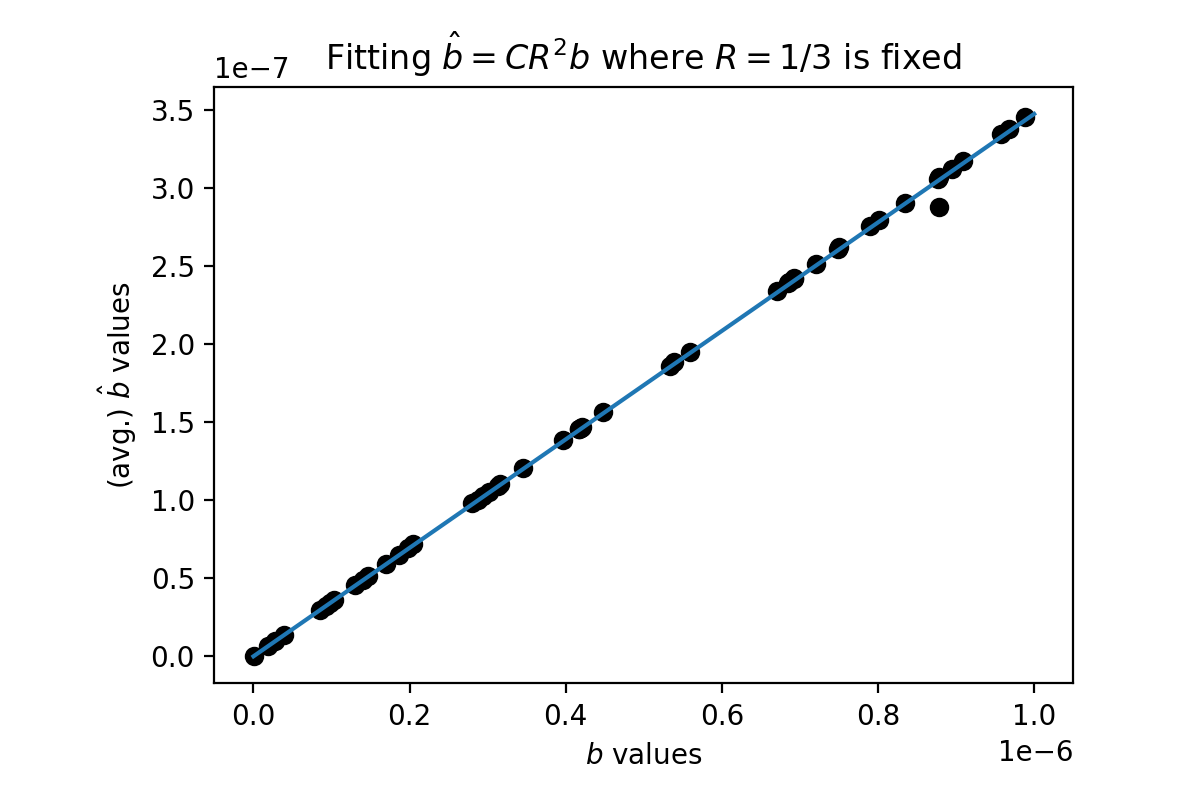
\includegraphics[width=\textwidth, trim={0cm 0 0cm 0}, clip]{kam_approx_line.png}
%
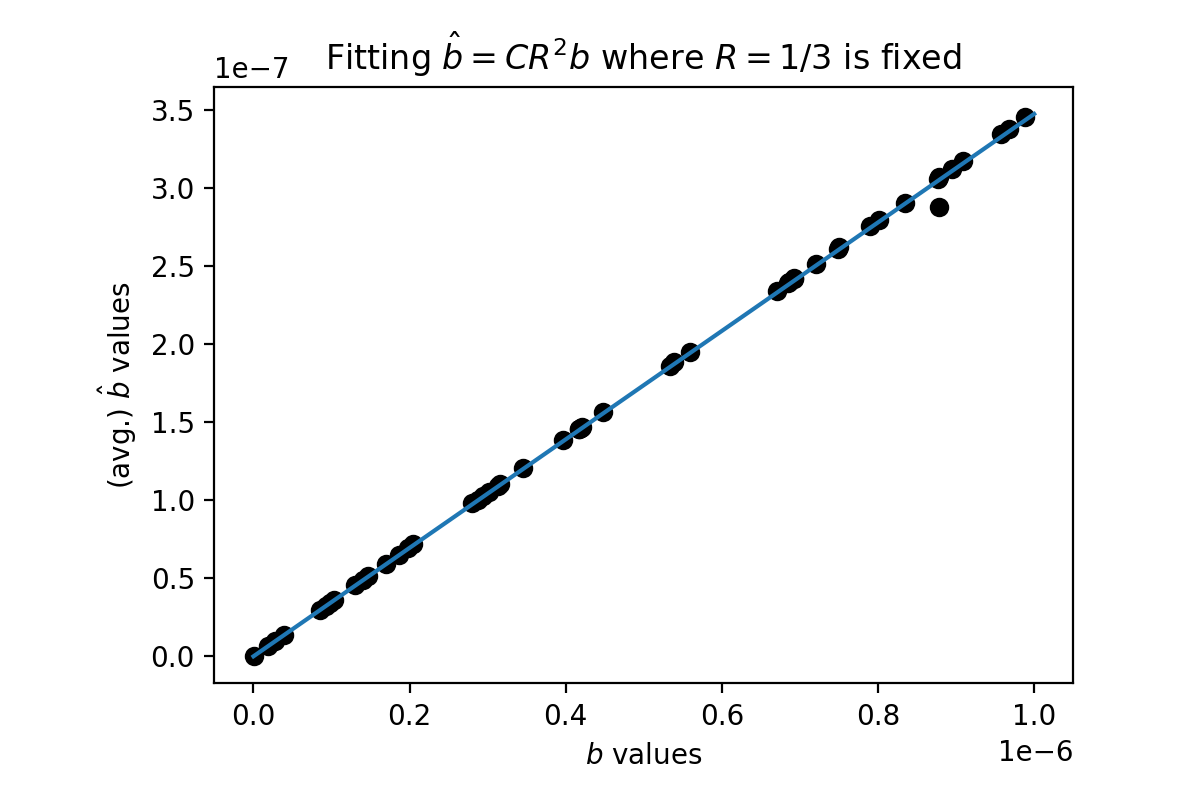
\includegraphics[width=\textwidth, trim={0cm 0 0cm 0}, clip]{kam_approx_line.png}
\caption{placeholder}
\end{subfigure}
\hfill
\caption{}
\end{figure}